\documentclass[../Cours.tex]{subfiles}

\begin{document}
\clearpage
\thispagestyle{empty}
\color{black}

\titreDScorrection

\begin{questions}
    \EXERCICE{4}
        \question
        \begin{itemize}
            \item On choisit 3
            \item On multiplie par 2 $\Rightarrow 3 \times 2 = 6$
            \item On ajoute au résultat 7 $\Rightarrow 6 + 7 = 13 $
            \item On multiplie le résultat par 8 $\Rightarrow 13 \times 8 = 104$
        \end{itemize}
        \question
        \begin{itemize}
            \item On choisit $\dfrac{5}{4}$
            \item On l'inverse : $\dfrac{4}{5}$
            \item On ajoute $\dfrac{1}{2} \Rightarrow \dfrac{4}{5} + \dfrac{1}{2} = \dfrac{8}{10} + \dfrac{5}{10} = \dfrac{13}{10}$
            \item On multiplie par $\dfrac{2}{3} \Rightarrow \dfrac{13}{10} \times \dfrac{2}{3} = \dfrac{26}{30}$
        \end{itemize}
        \question\\
        \underline{Dans le programme A :} 
        \begin{itemize}
            \item On choisit 1
            \item On multiplie par 2 $\Rightarrow 1 \times 2 = 2$
            \item On ajoute au résultat 7 $\Rightarrow 2 + 7 = 9 $
            \item On multiplie le résultat par 8 $\Rightarrow 9 \times 8 = 72$
        \end{itemize}
        \underline{Dans le programme B :}
        \begin{itemize}
            \item On choisit $\dfrac{2}{215}$
            \item On l'inverse : $\dfrac{215}{2}$
            \item On ajoute $\dfrac{1}{2} \Rightarrow \dfrac{215}{2} + \dfrac{1}{2} = \dfrac{216}{2} = 108$
            \item On multiplie par $\dfrac{2}{3} \Rightarrow 108 \times \dfrac{2}{3} = 72$
        \end{itemize}

        On trouve bien le même résultat dans les deux programmes : 72.

    \EXERCICE{6}
        \question Le triangle $ABC$ est rectangle en $B$, l'hypoténuse est $[AC]$.\\
        D'après le théorème de Pythagore :
        $$AC^2 = AB^2 + BC^2$$
        $$AC^2 = (3,1)^2 + (6,2)^2$$
        $$AC^2 = 9,61 + 38,44$$
        $$AC^2 = 48,05$$
        $$AC = \sqrt{48,05} \approx \qty{6,93}{\centi\metre}$$

        \clearpage
        \question 
        Dans un premier temps, faisons un schéma du problème :\\
        \begin{center}
            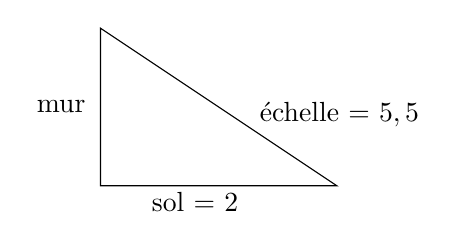
\begin{tikzpicture}
                \draw (0,0) -- (3,0) -- (0,2) -- cycle;
                \node at (1.2,-0.2) {sol = \qty{2}{\metre}};
                \node at (-0.5,1) {mur};
                \node[anchor=west] at (1.9,0.9) {échelle = $\qty{5,5}{\metre}$};
            \end{tikzpicture}
        \end{center}

        Il s'agit bien d'un triangle, il est rectangle parce que le mur est perpendiculaire au sol.
        On va donner un nom à ce triangle (on peut choisir les lettres que l'on veut, cela n'a aucune importance).\\
        Appelons ce triangle $DEF$, avec $DE = \qty{2}{\metre}$ et $EF = \qty{5,5}{\metre}$. On cherche donc la distance DF.\\
        \begin{enumerate}[label=\arabic*)]
            \item Le triangle $DEF$ est rectangle en $D$, l'hypoténuse est $[EF]$.
            \item D'après le théorème de Pythagore :
            \item $$EF^2 = DE^2 + DF^2$$
            \item $$(5,5)^2 = 2^2 + DF^2$$
            $$ DF^2 = (5,5)^2 - 2^2 $$
            $$ DF^2 = 30,25 - 4 = 26,25 $$
            $$ DF = \sqrt{26,25} \approx \qty{5,12}{\metre} $$
        \end{enumerate}

        Donc l'échelle pourra atteindre une hauteur de \qty{5,12}{\metre}.

    \EXERCICE{4}
        \question Il faut faire le calcul : $2 \times 1,20 + 3 \times 2,20$
        \question Cela donne : $2,40 + 6,60 = \qty{9}{\EURO}$
    Pierre va donc payer \qty{9}{\EURO} à la boulangerie.

    \EXERCICE{4}
    On calcule le volume du pavé droit : 
    $$V_{\mbox{pavé droit}} = L \times \ell \times h$$
    Cela donne 
    $$V_{\mbox{pavé droit}} = \qty{7}{\cm} \times \qty{3}{\cm} \times \qty{2}{\cm} = \qty{42}{\cm\cubed}$$

    On utilise un tableau de proportionnalité pour traduire la masse volumique \qty{10,50}{\g\per\cm\cubed}. En effet, \qty{10,50}{\g\per\cm\cubed} signifie que \qty{1}{\cm\cubed} d'argent pèse \qty{10,50}{\g} :

    \begin{center}
    \begin{tabularx}{0.4\linewidth}{|l|X|X|}\hline
        masse (\unit{\g}) & \num{10,50} & \\\hline
        volume (\unit{\cm\cubed}) & \num{1} & \\\hline
    \end{tabularx}
    \end{center}

    On complète le tableau avec la valeur du volume du pavé droit que l'on a calculé précédemment :
    
    \begin{center}
    \begin{tabularx}{0.4\linewidth}{|l|X|X|}\hline
        masse (\unit{\g}) & \num{10,50} & \\\hline
        volume (\unit{\cm\cubed}) & \num{1} & \num{42} \\\hline
    \end{tabularx}
    \end{center}

    Pour trouver la masse, on complète le tableau de proportionnalité en multipliant par $42$ pour passer de la première colonne à la deuxième colonne : (\textit{note : il y a d'autres méthodes pour faire ce genre de calcul, par exemple le produit en croix)}

    \begin{center}
    \begin{tikzpicture}
        \node at (0,0) {%
            \begin{tabularx}{0.4\linewidth}{|l|X|X|}\hline
                masse (\unit{\g}) & \num{10,50} & \\\hline
                volume (\unit{\cm\cubed}) & \num{1} & \num{42} \\\hline
            \end{tabularx}
        };%
        \draw[-Latex] (0.3,0.6) arc (180:0:0.8 and 0.5);
        \draw[-Latex] (0.3,-0.6) arc (180:360:0.8 and 0.5);*
        \node at (1.1,1.3) {$\times~42$};
        \node at (1.1,-1.3) {$\times~42$};
    \end{tikzpicture}
    \end{center}

    Donc la masse du pavé droit en argent est de $10,50 \times 42 = \qty{441}{\g}$.

    \EXERCICE{2} On souhaite déterminer le 278ème chiffre après la virgule de $\dfrac{16,3}{999}$.\\

    En utilisant la calculatrice, ou en posant la division, on remarque que :
    $\dfrac{16,3}{999} = \num{0,016 316 316 316 316}...$

    Mis à part le premier chiffre après la virgule qui est un 0, on remarque une récurrence : les mêmes trois chiffres 1, 6, 3 se répètent à l'infini dans cet ordre.

    Le 3ème chiffre après la virgule est un 6, le 6ème chiffre après la virgule est un 6, le 9ème aussi, le 12ème aussi, etc. C'est-à-dire que si le numéro du chiffre après la virgule est un multiple de 3, alors ce sera un 6.

    En l'occurrence, 276 est un multiple de 3 (car $2 + 7 + 6 = 15$ est dans la table de 3), donc le 276ème chiffre est un 6.

    On en déduit que le 277ème chiffre après la virgule est un 3, \textbf{donc le 278ème chiffre après la virgule est un 1.}
    
\end{questions}

\end{document}